\batchmode
\documentclass[11pt]{report}
\RequirePackage{ifthen}


\usepackage[pdftex,            pdfauthor={Jeffrey Yoo Warren},            pdftitle={Grassroots Mapping: a toolkit for participatory and activist cartography},            pdfsubject={Participatory Cartography},            pdfkeywords={Cartography},            pdfproducer={Latex with hyperref},            pdfcreator={pdflatex,colorlinks}]{hyperref}
\usepackage{graphicx,wrapfig,color,pdfcomment,booktabs,ctable,textcomp,tabularx,array,acronym,threeparttable}
\usepackage[table]{xcolor}
\usepackage[hang,small,bf,margin=0.5cm,tableposition=top]{caption}
\usepackage[ragged]{footmisc}%
\providecommand{\otoprule}{\midrule[\heavyrulewidth]} 
\definecolor{linkblue}{rgb}{0.2,0.2,1}
\hypersetup{colorlinks=true,
	    urlcolor=linkblue,
	    citecolor=linkblue,
	    linkcolor=linkblue}
\newcolumntype{Y}{>{\raggedright\arraybackslash}X}
\newcolumntype{W}{>{\raggedleft\arraybackslash}X}


\definecolor{tableShade}{HTML}{EEEEEE}


\title{Grassroots Mapping: a toolkit for participatory and politically engaged cartography}
\author{Jeffrey Warren}
\date{May 8, 2010}


\makeatletter

\makeatother
\urlstyle{jeff}





\pagecolor[gray]{.7}

\usepackage[]{inputenc}



\makeatletter

\makeatletter
\count@=\the\catcode`\_ \catcode`\_=8 
\newenvironment{tex2html_wrap}{}{}%
\catcode`\<=12\catcode`\_=\count@
\newcommand{\providedcommand}[1]{\expandafter\providecommand\csname #1\endcsname}%
\newcommand{\renewedcommand}[1]{\expandafter\providecommand\csname #1\endcsname{}%
  \expandafter\renewcommand\csname #1\endcsname}%
\newcommand{\newedenvironment}[1]{\newenvironment{#1}{}{}\renewenvironment{#1}}%
\let\newedcommand\renewedcommand
\let\renewedenvironment\newedenvironment
\makeatother
\let\mathon=$
\let\mathoff=$
\ifx\AtBeginDocument\undefined \newcommand{\AtBeginDocument}[1]{}\fi
\newbox\sizebox
\setlength{\hoffset}{0pt}\setlength{\voffset}{0pt}
\addtolength{\textheight}{\footskip}\setlength{\footskip}{0pt}
\addtolength{\textheight}{\topmargin}\setlength{\topmargin}{0pt}
\addtolength{\textheight}{\headheight}\setlength{\headheight}{0pt}
\addtolength{\textheight}{\headsep}\setlength{\headsep}{0pt}
\setlength{\textwidth}{349pt}
\newwrite\lthtmlwrite
\makeatletter
\let\realnormalsize=\normalsize
\global\topskip=2sp
\def\preveqno{}\let\real@float=\@float \let\realend@float=\end@float
\def\@float{\let\@savefreelist\@freelist\real@float}
\def\liih@math{\ifmmode$\else\bad@math\fi}
\def\end@float{\realend@float\global\let\@freelist\@savefreelist}
\let\real@dbflt=\@dbflt \let\end@dblfloat=\end@float
\let\@largefloatcheck=\relax
\let\if@boxedmulticols=\iftrue
\def\@dbflt{\let\@savefreelist\@freelist\real@dbflt}
\def\adjustnormalsize{\def\normalsize{\mathsurround=0pt \realnormalsize
 \parindent=0pt\abovedisplayskip=0pt\belowdisplayskip=0pt}%
 \def\phantompar{\csname par\endcsname}\normalsize}%
\def\lthtmltypeout#1{{\let\protect\string \immediate\write\lthtmlwrite{#1}}}%
\newcommand\lthtmlhboxmathA{\adjustnormalsize\setbox\sizebox=\hbox\bgroup\kern.05em }%
\newcommand\lthtmlhboxmathB{\adjustnormalsize\setbox\sizebox=\hbox to\hsize\bgroup\hfill }%
\newcommand\lthtmlvboxmathA{\adjustnormalsize\setbox\sizebox=\vbox\bgroup %
 \let\ifinner=\iffalse \let\)\liih@math }%
\newcommand\lthtmlboxmathZ{\@next\next\@currlist{}{\def\next{\voidb@x}}%
 \expandafter\box\next\egroup}%
\newcommand\lthtmlmathtype[1]{\gdef\lthtmlmathenv{#1}}%
\newcommand\lthtmllogmath{\dimen0\ht\sizebox \advance\dimen0\dp\sizebox
  \ifdim\dimen0>.95\vsize
   \lthtmltypeout{%
*** image for \lthtmlmathenv\space is too tall at \the\dimen0, reducing to .95 vsize ***}%
   \ht\sizebox.95\vsize \dp\sizebox\z@ \fi
  \lthtmltypeout{l2hSize %
:\lthtmlmathenv:\the\ht\sizebox::\the\dp\sizebox::\the\wd\sizebox.\preveqno}}%
\newcommand\lthtmlfigureA[1]{\let\@savefreelist\@freelist
       \lthtmlmathtype{#1}\lthtmlvboxmathA}%
\newcommand\lthtmlpictureA{\bgroup\catcode`\_=8 \lthtmlpictureB}%
\newcommand\lthtmlpictureB[1]{\lthtmlmathtype{#1}\egroup
       \let\@savefreelist\@freelist \lthtmlhboxmathB}%
\newcommand\lthtmlpictureZ[1]{\hfill\lthtmlfigureZ}%
\newcommand\lthtmlfigureZ{\lthtmlboxmathZ\lthtmllogmath\copy\sizebox
       \global\let\@freelist\@savefreelist}%
\newcommand\lthtmldisplayA{\bgroup\catcode`\_=8 \lthtmldisplayAi}%
\newcommand\lthtmldisplayAi[1]{\lthtmlmathtype{#1}\egroup\lthtmlvboxmathA}%
\newcommand\lthtmldisplayB[1]{\edef\preveqno{(\theequation)}%
  \lthtmldisplayA{#1}\let\@eqnnum\relax}%
\newcommand\lthtmldisplayZ{\lthtmlboxmathZ\lthtmllogmath\lthtmlsetmath}%
\newcommand\lthtmlinlinemathA{\bgroup\catcode`\_=8 \lthtmlinlinemathB}
\newcommand\lthtmlinlinemathB[1]{\lthtmlmathtype{#1}\egroup\lthtmlhboxmathA
  \vrule height1.5ex width0pt }%
\newcommand\lthtmlinlineA{\bgroup\catcode`\_=8 \lthtmlinlineB}%
\newcommand\lthtmlinlineB[1]{\lthtmlmathtype{#1}\egroup\lthtmlhboxmathA}%
\newcommand\lthtmlinlineZ{\egroup\expandafter\ifdim\dp\sizebox>0pt %
  \expandafter\centerinlinemath\fi\lthtmllogmath\lthtmlsetinline}
\newcommand\lthtmlinlinemathZ{\egroup\expandafter\ifdim\dp\sizebox>0pt %
  \expandafter\centerinlinemath\fi\lthtmllogmath\lthtmlsetmath}
\newcommand\lthtmlindisplaymathZ{\egroup %
  \centerinlinemath\lthtmllogmath\lthtmlsetmath}
\def\lthtmlsetinline{\hbox{\vrule width.1em \vtop{\vbox{%
  \kern.1em\copy\sizebox}\ifdim\dp\sizebox>0pt\kern.1em\else\kern.3pt\fi
  \ifdim\hsize>\wd\sizebox \hrule depth1pt\fi}}}
\def\lthtmlsetmath{\hbox{\vrule width.1em\kern-.05em\vtop{\vbox{%
  \kern.1em\kern0.8 pt\hbox{\hglue.17em\copy\sizebox\hglue0.8 pt}}\kern.3pt%
  \ifdim\dp\sizebox>0pt\kern.1em\fi \kern0.8 pt%
  \ifdim\hsize>\wd\sizebox \hrule depth1pt\fi}}}
\def\centerinlinemath{%
  \dimen1=\ifdim\ht\sizebox<\dp\sizebox \dp\sizebox\else\ht\sizebox\fi
  \advance\dimen1by.5pt \vrule width0pt height\dimen1 depth\dimen1 
 \dp\sizebox=\dimen1\ht\sizebox=\dimen1\relax}

\def\lthtmlcheckvsize{\ifdim\ht\sizebox<\vsize 
  \ifdim\wd\sizebox<\hsize\expandafter\hfill\fi \expandafter\vfill
  \else\expandafter\vss\fi}%
\providecommand{\selectlanguage}[1]{}%
\makeatletter \tracingstats = 1 


\begin{document}
\pagestyle{empty}\thispagestyle{empty}\lthtmltypeout{}%
\lthtmltypeout{latex2htmlLength hsize=\the\hsize}\lthtmltypeout{}%
\lthtmltypeout{latex2htmlLength vsize=\the\vsize}\lthtmltypeout{}%
\lthtmltypeout{latex2htmlLength hoffset=\the\hoffset}\lthtmltypeout{}%
\lthtmltypeout{latex2htmlLength voffset=\the\voffset}\lthtmltypeout{}%
\lthtmltypeout{latex2htmlLength topmargin=\the\topmargin}\lthtmltypeout{}%
\lthtmltypeout{latex2htmlLength topskip=\the\topskip}\lthtmltypeout{}%
\lthtmltypeout{latex2htmlLength headheight=\the\headheight}\lthtmltypeout{}%
\lthtmltypeout{latex2htmlLength headsep=\the\headsep}\lthtmltypeout{}%
\lthtmltypeout{latex2htmlLength parskip=\the\parskip}\lthtmltypeout{}%
\lthtmltypeout{latex2htmlLength oddsidemargin=\the\oddsidemargin}\lthtmltypeout{}%
\makeatletter
\if@twoside\lthtmltypeout{latex2htmlLength evensidemargin=\the\evensidemargin}%
\else\lthtmltypeout{latex2htmlLength evensidemargin=\the\oddsidemargin}\fi%
\lthtmltypeout{}%
\makeatother
\setcounter{page}{1}
\onecolumn

% !!! IMAGES START HERE !!!

\stepcounter{chapter}
\stepcounter{section}
\stepcounter{subsection}
\stepcounter{subsection}
\stepcounter{subsection}
\stepcounter{section}
{\newpage\clearpage
\lthtmlfigureA{table43}%
\begin{table}
\centering %
\renewedcommand{arraystretch}{1.4}
\begin{tabularx}{\textwidth}{YYY}
\toprule
Capture&Orthorectification&Publication\\\midrule[\heavyrulewidth]
2-3 people can map several square km in 1 day&Sorting photos can take \textgreater1 hour, stitching up to 1 day&Export from Cartagen Knitter generates a TMS or printable GeoTiff; only web access is needed.\\\bottomrule 
\end{tabularx}
\end{table}%
\lthtmlfigureZ
\lthtmlcheckvsize\clearpage}

\stepcounter{chapter}
\stepcounter{section}
\stepcounter{section}
\stepcounter{section}
\stepcounter{chapter}
\stepcounter{section}
\stepcounter{section}
\stepcounter{subsection}
\stepcounter{subsection}
\stepcounter{section}
\stepcounter{section}
\stepcounter{section}
\stepcounter{chapter}
\stepcounter{section}
\stepcounter{section}
\stepcounter{subsection}
\stepcounter{section}
\stepcounter{subsection}
\stepcounter{subsubsection}
\stepcounter{subsubsection}
\stepcounter{chapter}
\stepcounter{subsection}
\stepcounter{subsection}
\stepcounter{section}
\stepcounter{subsection}
\stepcounter{section}
\stepcounter{subsection}
\stepcounter{subsection}
\stepcounter{subsubsection}
\stepcounter{subsubsection}
\stepcounter{section}
\stepcounter{subsection}
\stepcounter{subsection}
\stepcounter{subsection}
\stepcounter{section}
\stepcounter{chapter}
\stepcounter{section}
{\newpage\clearpage
\lthtmlfigureA{table362}%
\begin{table}
\par
\centering %
\rowcolors{1}{tableShade}{white}
\renewedcommand{arraystretch}{1.4}
\begin{tabularx}{\textwidth}{>{\bfseries }rYY}
\toprule\hiderowcolors
Type&Kite&Balloon\\\midrule[\heavyrulewidth]\showrowcolors
Altitude&300m&1400m\\
Extent&several hundred meters&\textgreater1km is common\\
Control&hard to target imagery - difficult in winds \textless45kph or \textless10kph&very fine control on windless days - difficult in winds \textgreater10kph\\
Payload&\textless2 kg&\textless300g\\
Time constraints&best winds in early afternoon&lowest winds at dawn\\
Portability&foil kites pack down to 1 liter size&helium tank and fragility of balloon limit portability, access\\
Tether angle&poor, camera altitude as low as 1/5 of tether length&in windless conditions, flies vertically; very sensitive to wind\\
Durability&excellent, no consumables&very poor; balloons pop regularly\\
Cost per flight&none&\$15-35 per flight dependent on helium costs\\
Initial total cost of kit&\$60-400 depending on kite and tether material&\$100-500 depending on choice of balloon and tether material\\\bottomrule
\end{tabularx}
\end{table}%
\lthtmlfigureZ
\lthtmlcheckvsize\clearpage}

\stepcounter{subsection}
{\newpage\clearpage
\lthtmlfigureA{table384}%
\begin{table}\begin{threeparttable}[b]

\centering %
\rowcolors{1}{tableShade}{white}
\renewedcommand{arraystretch}{1.4}
\begin{tabularx}{\textwidth}{>{\bfseries }WYYY}
\toprule\hiderowcolors
Type&Cost&Typical \# of uses&Permeability\\\midrule[\heavyrulewidth]\showrowcolors
5-foot polyurethane advertising balloon\tnote{1}&\$US 140&hundreds?&Deflates 1-3\% per day\\
8-foot\tnote{2} latex weather balloon&\$US 25&up to 10 if careful&remains inflated for several hours; this weakens the balloon\\
Trash bags&~\$US 2&2-3&1-2 days if thicker (3 mil) plastic is used\\\bottomrule 
\end{tabularx}
\begin{tablenotes}
\item [1] Available from Southern Balloon Works, \url{southernballoonworks.com}
\item [2] `8-foot' denotes burst diameter, actual filled diameter during use is approximately 4 feet
\end{tablenotes}
\end{threeparttable}
\end{table}%
\lthtmlfigureZ
\lthtmlcheckvsize\clearpage}

\stepcounter{subsection}
\stepcounter{subsection}
\stepcounter{subsection}
\stepcounter{section}
\stepcounter{subsection}
\stepcounter{subsubsection}
\stepcounter{section}
\stepcounter{subsection}
\stepcounter{subsection}
\stepcounter{subsection}
\stepcounter{chapter}
\stepcounter{section}
\stepcounter{subsection}
\stepcounter{subsection}
\stepcounter{subsubsection}
\stepcounter{subsubsection}
\stepcounter{subsubsection}
\stepcounter{subsection}
\stepcounter{subsection}
\stepcounter{subsubsection}
\stepcounter{subsubsection}
{\newpage\clearpage
\lthtmlfigureA{table613}%
\begin{table} 
\par
\centering %
\rowcolors{1}{tableShade}{white}
\renewedcommand{arraystretch}{1.4}
\begin{tabularx}{\textwidth}{>{\bfseries }rlYYY}
\toprule\hiderowcolors
Site&Criteria&Grassroots Mapping&Google Maps&Percent change\\\midrule[\heavyrulewidth]\showrowcolors
Juan Pablo II&Resolution&&&\\
&Recency&&&\\
&Roof count&107&66&+62\%\\\hline
San Ignacio Loyola&Resolution&&&\\
&Recency&&&\\
&Roof count&&&\\\hline
Canta Gallo&Resolution&29cm&7cm&+411\%\\
&Recency&&&\\
&Roof count&&&\\
\bottomrule
\end{tabularx}
\end{table}%
\lthtmlfigureZ
\lthtmlcheckvsize\clearpage}

\stepcounter{subsection}
\stepcounter{subsection}
\stepcounter{chapter}
\stepcounter{section}
\stepcounter{section}
\stepcounter{section}
\stepcounter{section}
\stepcounter{subsection}
\stepcounter{subsection}
\stepcounter{subsection}
\stepcounter{subsection}
\stepcounter{section}
\stepcounter{section}
\stepcounter{section}
\stepcounter{section}
\stepcounter{section}
{\newpage\clearpage
\lthtmlfigureA{table689}%
\begin{table}
\par
\centering %
\rowcolors{1}{tableShade}{white}
\renewedcommand{arraystretch}{1.0}
\begin{tabularx}{\textwidth}{lYYY}
\toprule\hiderowcolors
Conditions&Balloon or Kite&\# of images&Est. max altitude (ft)\\\midrule[\heavyrulewidth]\showrowcolors
&balloon&222&1500\\
&kite&184&\\
&kite&54&\\
&balloon&318&\\
steady wind grew to 20 mph&kite&200&1000\\
&balloon&118&\\
&balloon&182&\\
windy&balloon&100&350\\
very windy&kite&&300\\
good wind&kite&&1000\\
lots of wind&kite&&1000\\
good wind&kite&&1000\\
good&balloon&124&750\\
good&balloon&&350\\
7-8 mph&balloon&362&300\\
poor wind&kite&&500\\
very windy&both&213&1000/1000\\
good&balloon&&800\\
&balloon&665&700\\
stormy&balloon&&1000\\
low wind&kite&&200\\
7-8 mph&balloon&&400\\
very windy&kite&&\\
windy&kite&472&350\\
low wind&both&166&\\
windy&kite&398&350\\
&kite&200&\\
mild steady wind&balloon&323&400\\
difficult wind&balloon&1000&500\\
&balloon&900&300-600\\
wind in wrong direction&balloon&50&500\\
&kite&325&\\
good wind&balloon&971&1000\\
\bottomrule
\end{tabularx}
\end{table}%
\lthtmlfigureZ
\lthtmlcheckvsize\clearpage}

{\newpage\clearpage
\lthtmlfigureA{table702}%
\begin{table} 
\par
\centering %
\rowcolors{1}{tableShade}{white}
\renewedcommand{arraystretch}{1.4}
\begin{tabularx}{\textwidth}{>{\bfseries }rlYYYYYY}
\toprule\hiderowcolors
Site&Coordinates&Date of capture&Resolution&Area&Trip Leader&Estimated altitude&Technique\\\midrule[\heavyrulewidth]\showrowcolors
Grand Isle State Park&&&&&&&\\\hline
Grand Isle State Park&&&&&&&\\
\bottomrule
\end{tabularx}
\end{table}%
\lthtmlfigureZ
\lthtmlcheckvsize\clearpage}

\stepcounter{section}
\stepcounter{chapter}
\stepcounter{section}
\stepcounter{section}
\stepcounter{subsubsection}
\stepcounter{subsubsection}
\stepcounter{subsubsection}
\stepcounter{subsubsection}
\stepcounter{subsection}
\stepcounter{section}
\stepcounter{section}
\stepcounter{subsection}
{\newpage\clearpage
\lthtmlpictureA{tex2html_wrap5741}%
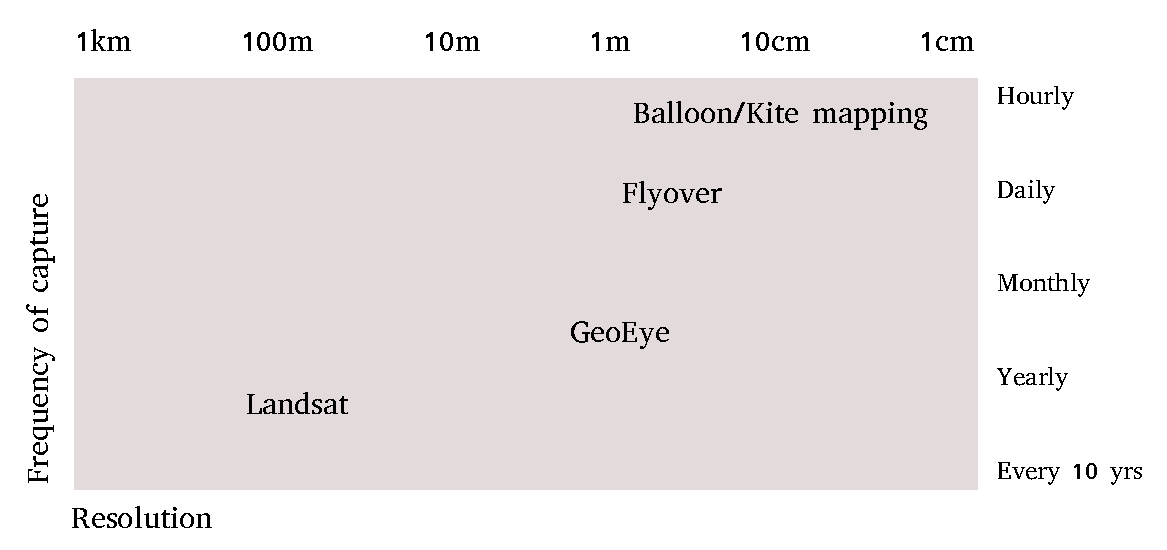
\includegraphics[width=1\textwidth]{diagrams/resolution-frequency.pdf}%
\lthtmlpictureZ
\lthtmlcheckvsize\clearpage}

\stepcounter{subsection}
\stepcounter{subsection}
\stepcounter{subsection}
\stepcounter{chapter}
\stepcounter{section}
\stepcounter{subsection}
\stepcounter{subsection}
\stepcounter{section}
\stepcounter{section}
\stepcounter{section}
\appendix
\stepcounter{chapter}
\stepcounter{section}
\stepcounter{subsection}
\stepcounter{subsection}
\stepcounter{subsection}
\stepcounter{subsection}
\stepcounter{section}
\stepcounter{section}
\stepcounter{subsection}
\stepcounter{subsection}
\stepcounter{section}
\stepcounter{chapter}
\stepcounter{chapter}
\stepcounter{section}
{\newpage\clearpage
\lthtmlfigureA{table826}%
\begin{table}
\centering %
\renewedcommand{arraystretch}{1.4}
\begin{tabularx}{\textwidth}{YYY}
\toprule
Capture&Orthorectification&Publication\\\midrule[\heavyrulewidth]
2-3 people can map several square km in 1 day&Sorting photos can take \textgreater1 hour, stitching up to 1 day&Export from Cartagen Knitter generates a TMS or printable GeoTiff; only web access is needed.\\\bottomrule 
\end{tabularx}
\end{table}%
\lthtmlfigureZ
\lthtmlcheckvsize\clearpage}

\stepcounter{chapter}
{\newpage\clearpage
\lthtmlfigureA{acronym859}%
\begin{acronym}
\acro{TMS}{Tiled Map Service}
\acro{GeoTIFF}{Geographic TIFF, or Geographic Tiled Image File Format}
\acro{CHDK}{Canon Hacker Development Kit}
\acro{KAP}{Kite Aerial Photography}
\acro{BAP}{Balloon Aerial Photography}
\acro{COFOPRI}{Organization for the Formalization of Informal Property}
\acro{LABB}{Louisiana Bucket Brigade}
\end{acronym}%
\lthtmlfigureZ
\lthtmlcheckvsize\clearpage}


\end{document}
